\subsubsection{Система динамического управление}\label{part_dynamic_control}

Каждый из приводов манипулятора робота Kuka Youbot имеет собственную систему управления, структура которой иллюстрируется схемой с рисунка~\ref{img_structure_of_actuator_cs}.
Из нее видно, что каждый из приводов робота может управляться заданием значения для угла~$q_{di}$, или скорости~$\dot{q}_{di}$, или момента силы $\tau_{ed,i}$, который должен быть на нем обеспечен.
Это значение подается на вход соответствующего ПИД-регулятора, коэффициенты которого доступны настройке, и далее (уже в виде сигнала напряжения $u$)~--- на контролируемый двигатель.

\vspace{0.5cm}

\begin{figure}[h!]
	\centering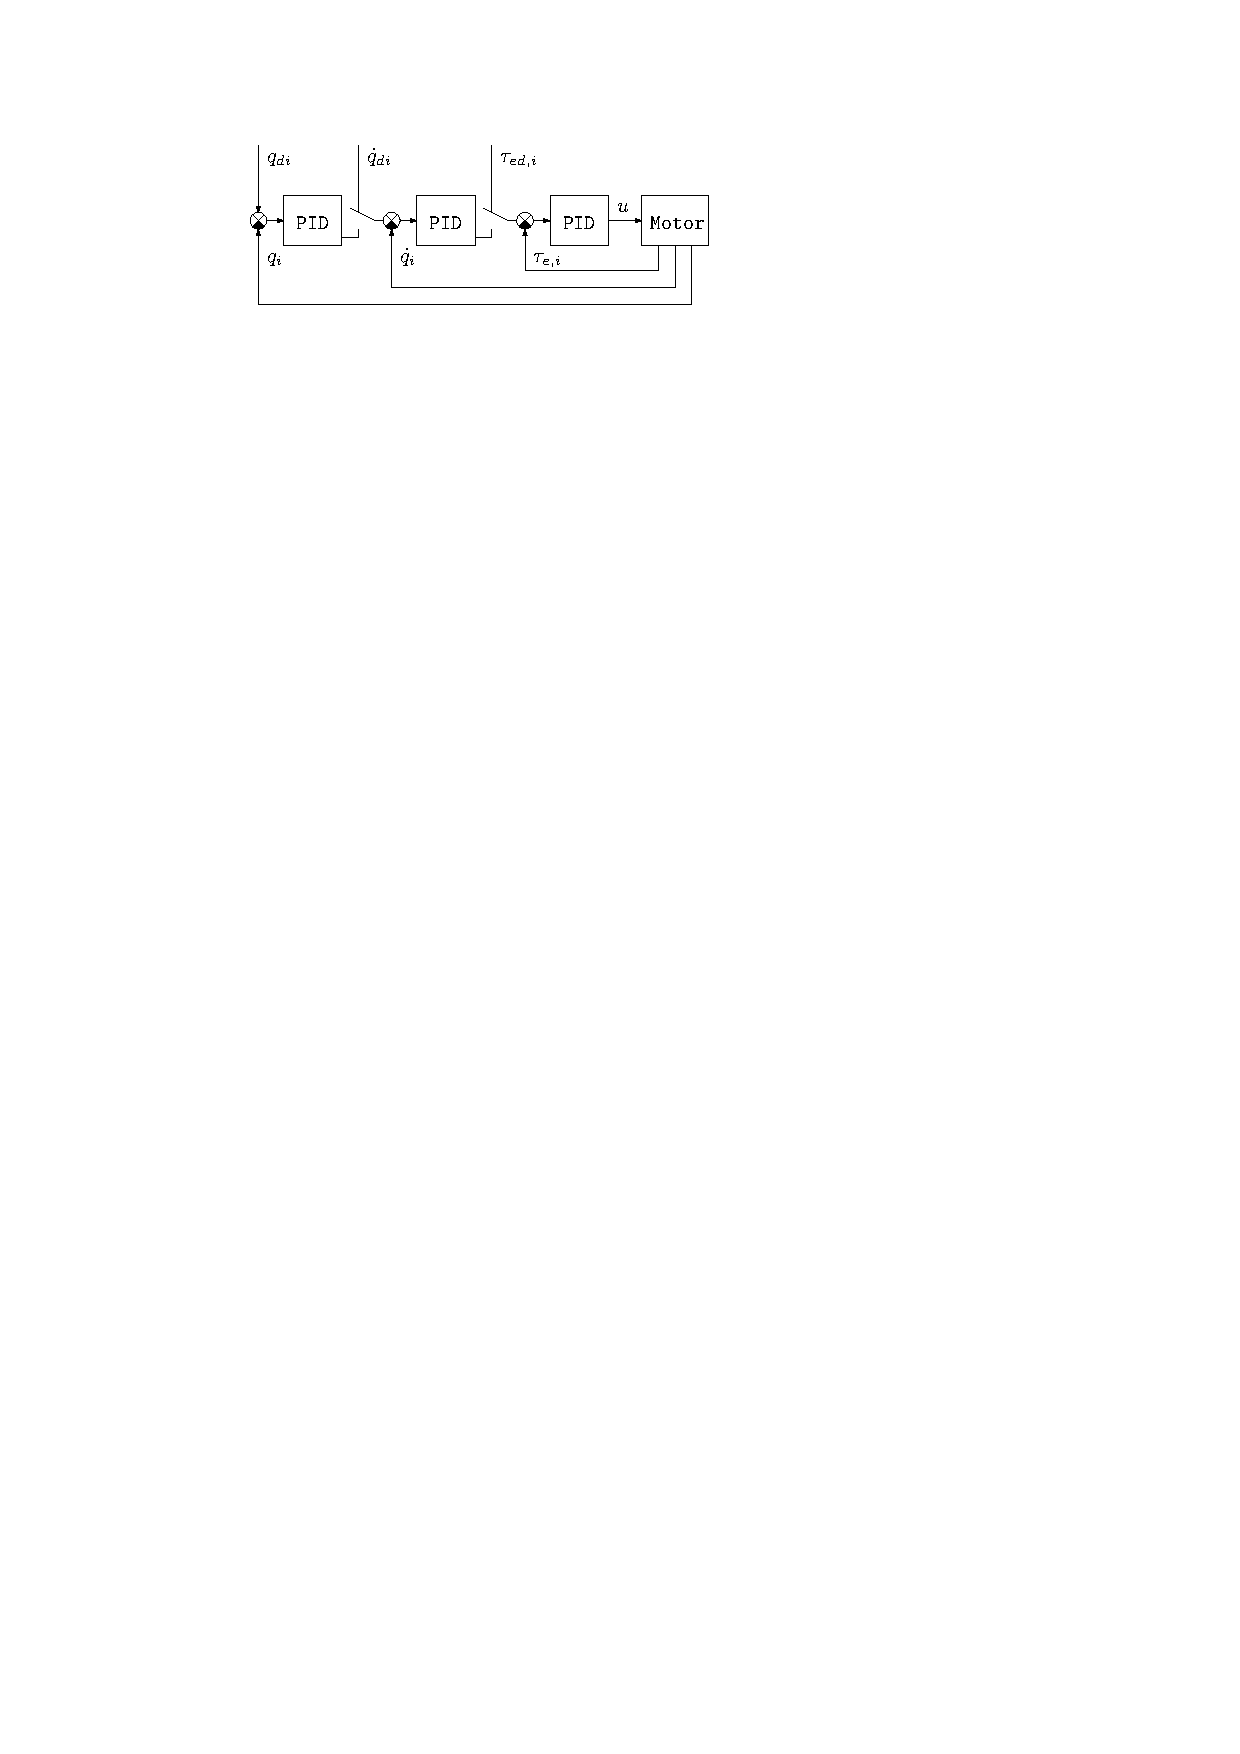
\includegraphics[width=0.8\textwidth]{structure_of_actuator_cs.pdf}
	\caption{Структура системы управления, контролирующей работу каждого из приводов робота.}
	\label{img_structure_of_actuator_cs}
\end{figure}

Далее в тексте документа будут рассмотрены системы управления, в которых в качестве управляющего сигнала рассматривается вектор $\tau_e(t)$.
При этом будет предполагаться, что задаваемые значения для моментов сил достигаются на двигателях мгновенно.
Такое предположение будем считать возможным по той причине, что процессы в контуре момента в рассмотренной выше системе управления характеризуются малыми временами переходных процессов.
В~качестве иллюстрации к сказанному можно привести рисунок~\ref{img_pid_transition_function}.
На нем показан график переходной функции системы управления моментом силы, развиваемым приводом i-го звена.

Из величин, описывающих состояние робота в данный момент времени, в используемом ПО доступны вектора $q(t)$, $\dot{q}(t)$ и $\tau_e(t)$.


\textbf{Система управления для принятия определенной конфигурации}

Для системы управления процессом принятия роботом желаемой конфигурации, описываемой вектором $q_d = \left[ q_{d1} \; q_{d2} \; q_{d3} \; q_{d4} \; q_{d5} \right]^T = const$, выберем следующий закон управления:
\begin{equation}\label{eq_set_point_control_law}
    \tau_e = K_p (q_d - q) - K_d \dot{q} + G(q) + t_f(\dot{q}),
\end{equation}
где $K_p = \diag\{k_{pi}\} = const$ и $K_d = \diag\{k_{di}\} = const$, при этом $k_{pi}>0$ и $k_{di}>0$ для $\forall i=\overline{1,5}$.
С~учетом его и уравнения~\eqref{eq_model_with_standard_matrix} модель замкнутой системы примет вид:
\begin{equation}
    M(q) \ddot{q} + C(q,\dot{q}) \dot{q} = K_p (q_d - q) - K_d \dot{q}\ldotp
\end{equation}
Это выражение с использованием обозначений
\begin{equation}
    e = q - q_d,
    \qquad \qquad
    x =
    \begin{bmatrix}
        e \\ \dot{q}
    \end{bmatrix}\!\!,
\end{equation}
можно переписать следующим образом
\begin{equation}\label{eq_controlled_object_model}
    \dot{x} = f(x),
\end{equation}
где
\begin{equation}
    f(x) =
    \begin{bmatrix}
        \dot{q} \\
        -M^{-1}(e) \Bigl( K_p e + K_d \dot{q} + C(e,\dot{q}) \dot{q} \Bigr)
    \end{bmatrix}\!\!\ldotp
\end{equation}

Заметим, что равновесным состоянием системы~\eqref{eq_controlled_object_model} является точка \linebreak $x_0 = [0\;0\;\ldots\;0]^T$, так как $f(x_0) = [0\;0\;\ldots\;0]^T$.

Рассмотрим следующую функцию Ляпунова:
\begin{equation}
    V(x) = \frac{1}{2} \, \dot{q}^T \! M(e) \dot{q} + \frac{1}{2} \, e^T \! K_p e \ldotp
\end{equation}
Ее производная по времени\footnote{В~представленных ниже выкладках учтен тот факт, что матрица \linebreak $\bigl( 0.5 M(q) \bigr)^\centerdot \!\! - C(q,\dot{q})$ является кососимметричной.}
\begin{gather}
    \frac{d}{dt} V(x) = \dot{q}^T \! M(e) \ddot{q} + \dot{q}^T \frac{d}{dt} \Bigl( \frac{1}{2} M(e) \Bigr) \dot{q} + \dot{e}^T K_p e = \notag \\
    %
    = \dot{q}^T \Bigl( \tau_e - C(q,\dot{q}) \dot{q} - G(q) - t_f(\dot{q}) \Bigr) + \dot{q}^T \frac{d}{dt} \Bigl( \frac{1}{2} M(q) \Bigr) \dot{q} + \dot{q}^T K_p e  = \notag\\
    %
    = \dot{q}^T \Bigl( \tau_e - G(q) - t_f(\dot{q}) + K_p e\Bigr) + \dot{q}^T \biggl( \frac{d}{dt} \Bigl( \frac{1}{2} M(q) \Bigr) - C(q,\dot{q}) \biggr) \dot{q} = \notag \\
    %
    = \dot{q}^T \Bigl(K_p (q_d - q) - K_d \dot{q} + G(q) + t_f(\dot{q}) - G(q) - t_f(\dot{q}) + K_p (q - q_d) \Bigr) = \notag \\
    %
    = -\dot{q}^T K_d \dot{q} < 0
\end{gather}
при $x \ne x_0$ и равна нулю при $x = x_0$.
Следовательно, по 2-ой теореме Ляпунова состояние системы $x = x_0$, при котором, к слову сказать, $q = q_d$ и $\dot{q} = [0\;0\;\ldots\;0]^T$, является асимптотически устойчивым.

\textbf{Система управления процессом следования по траектории}

Для системы управления процессом следования роботом по траектории, описываемой вектор-функцией $q_d(t) = \left[ q_{d1}(t) \; q_{d2}(t) \; q_{d3}(t) \; q_{d4}(t) \; q_{d5}(t) \right]^T$\!\!\!,\; возьмем следующий закон управления:
\begin{equation}\label{eq_trajectory_tracking_control_law}
    \tau_e = M(q) \bigl( \ddot{q}_d + K_d (\dot{q}_d - \dot{q})+  K_p (q_d - q) \bigr) + C(q,\dot{q}) \dot{q} + G(q) + t_f(\dot{q}),
\end{equation}
где $K_d = const$ и $K_p = const$.

С~учетом его и уравнения~\eqref{eq_model_with_standard_matrix} модель замкнутой системы опишется следующим выражением:
\begin{equation}
    M(q) \bigl( \ddot{q}_d - \ddot{q} + K_d (\dot{q}_d - \dot{q})+  K_p (q_d - q) \bigr) = 0,
\end{equation}
которое после деления на $M(q)$ и применения обозначения
\begin{equation}
    \varepsilon = q_d - q
\end{equation}
может быть переписано в виде:
\begin{equation}\label{eq_trajectory_tracking_closed_loop}
    \ddot{\varepsilon} + K_d \dot{\varepsilon} +  K_p \varepsilon = 0 \ldotp
\end{equation}

Согласно последнему уравнению, использование закона управления~\eqref{eq_trajectory_tracking_control_law} дает возможность полностью определять поведение робота значениями матриц $K_p$ и $K_d$.

В~данной работе матрицы $K_p$ и $K_d$ были выбраны диагональными:
\begin{equation}
    K_p = \diag\{k_{pi}\},
    \qquad
    K_d = \diag\{k_{di}\},
\end{equation}
потому что это позволяет <<разбить>> уравнение~\eqref{eq_trajectory_tracking_closed_loop} на 5~независимых дифференциальных уравнений, а их компоненты~--- положительными:
\begin{equation}
    \qquad
    k_{pi} > 0,\ k_{di} > 0,\ \forall i=\overline{1,5},
\end{equation}
так как при этом система получается устойчивой (все 5~уравнений получаются имеющими корни только с отрицательной вещественной частью).

\newpage
